\newpage
\begin{center}
  \textbf{\large 3. РАЗРАБОТКА СОБСТВЕННОГО МЕТОДА}
\end{center}
\refstepcounter{chapter}
\addcontentsline{toc}{chapter}{3. РАЗРАБОТКА СОБСТВЕННОГО МЕТОДА}

Наша основная идея в обучение языковой модели на русском языке для исправление ошибок.
Как мы обсуждали ранее, в основном методы, завязанные на LM полагаются на скрытое представление ASR модели или же на её проекцию в скрытое представление языковой модели.
Мы же будем проводить наши тесты с использованием естественного языка.
То есть мы будем сначала транскрибировать аудио в текст и только потом его править.
Таким образом мы решим проблему универсальности подхода и независимости ASR-LM пары.

\section{Генерация датасета}
Теперь необходимо создать датасет для обучения.
Для этого возьмём и сгенерируем 5 гипотез с помощью BeamSearch метода.
Затем мы подадим все 5 гипотез в нашу модель и попросим сгенерировать исправленную последовательность.

Почему подавать 5 гипотез в модель? Что мы можем взять из гипотез?
Почему просто не реранжировать гипотезы?
Давайте проанализируем полученные данные.

\textcolor{red}{Тут графки.}

Сначала разъясним, почему не реранжирование.
Первый график на Рис. 1 показывает процент случаев, когда гипотеза 2-5 имеют ниже WER, чем 1 гипотеза.
Их процент колеблется от 4 до 8, что значит мы можем не получить значительного прироста.
Второй график же показывает процент токенов, которые:
\begin{itemize}
  \item Есть в праильной транскрипции.
  \item Есть в гипотезе $n_k$ и нет в гипотезах $n_i$, где $i < k$.
\end{itemize}

Это та самая информация, которую наша модель может извлечь из сгенерированных гипотез и улучшить качество транскрипции.
Именно поэтом мы переходим к обучению отдельной языковой модели на ошибках.

\section{Описание моделей и процесса обучения}

T5 (Text-to-Text Transfer Transformer) -- это универсальная трансформерная модель, разработанная Google Research, которая переформулирует все задачи обработки естественного языка в единый формат Sequence-to-Sequence (Seq2Seq).
Её ключевая особенность -- подход, при котором задачи классификация, перевода, суммаризации и др. представляются как преобразование входной текстовой строки в выходную.

Модель использует энкодер-декодер структуру, где:
\begin{itemize}
  \item Энкодер обрабатывает входной текст, создавая контекстуализированные представления для каждого токена.
  В отличие от чисто декодерных моделей типа GPT, T5 использует двунаправленное внимание, что позволяет анализировать весь входной текст одновременно.
  \item Декодер генерирует выход последовательно, используя авторегрессионный механизм.
  При этом он учитывает скрытые состояния энкодера через кросс-внимание.
  Схожим образом работает ранее Whisper.
\end{itemize}

\begin{figure}[!t]
  \centering
  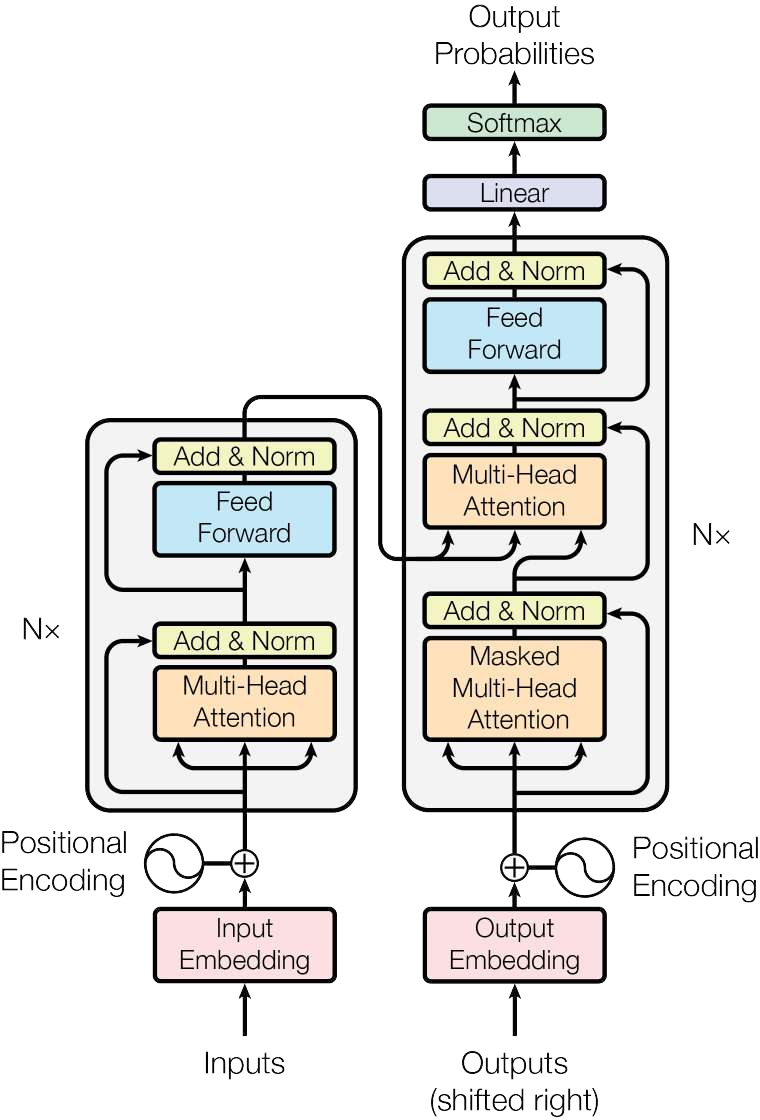
\includegraphics[width=80mm]{enc_dec.pdf}
  \caption{Архитектура энкодер-декодер.}
  \label{fig:enc_dec}
\end{figure}

Схема архитектуры представлена на Рис.~\ref{fig:enc_dec}

Универсальность подхода Seq2Seq позволяет применять одну и ту же модель для десятков задач без изменения архитектуры.

В качестве двух моделей мы возьмём ruT5 и Fred-T5.
Обе модели были обучены Сбером на корпусе русского языка.
Они построены на архитектуре энкодер-декодер трансформеров.
Их мы выбрали по нескольким причинам:

\begin{enumerate}
  \item \textbf{Размер}.
  Мы берём Base (220М) и distil (95М) версии соответственно. 
  В паре с FastConformer это займёт немногим больше 3 Гб видеопамяти, что позволит влезть в любую пользовательскую видеокарту.
  \item \textbf{Архитектура}.
  Энкодер-декодер лучше улавливает ошибки и корректирует их.
  Такие выводы были сделаны на основе решения этой задачи для английского языка, где в качестве моделей-корректоров использовались Mistral-7b и Llama3-8b.
  На русском они также показывают плохие результаты, поэтому включены они не были.
\end{enumerate}

Обучение ruT5 будет проходить в few-shot сценарии, когда мы ей будем показывать 3 примера из валидационной выборке в качестве примера для улучшения.
Few-shot -- это подход, при котором языковая модель решает новую задачу, используя несколько демонстрационных примеров.
Математически это можно выразить как~\ref{eq:shot}:

\begin{equation}
  P(y_{test}|x_{test},\{x_i,y_i\}^K_{i=1}) = \prod_{t=1}^{T}P(w_t|w_{<t},x_{test},\{(x_i,y_i)\}^K_{i=1},\theta)
  \label{eq:shot}
\end{equation}
где $w_t$ - t-й токен ответа, $T$ - длина ответа, а $\theta$ - параметры модели.

Так мы проведём 15 обучающих эпох и сохраним модель с наименьшим WER на валидационной выборке.
Дополнительн мы используем метод Low-rank adaptaion (LoRA).
Это метод, при котором изначальные веса модели в выбранных слоях замораживаются и никак не изменяются в ходе дообучения.
В нашем случае такими слоями будут слои attention.
У каждой матрицы attention (Q, K, V, O) инициализируется своя пара матриц A и B размерами (h, rank) и (rank, h), где h – размер скрытого пространства матрицы attention, а rank – размер ранга, заданный при LoRA.
Во время обучения будут изменяться как раз матрицы A и B, которые как бы представляют собой сжатую информацию из весов слоя.
Преимуществом LoRA является то, что мы значительно экономим в используемой памяти, жертвуя качеством.
Это происходит благодаря тому, что в state оптимизатора хранятся не матрицы размера h $\times$ h, а две матрицы размеров h $\times$ rank и rank $\times$ h.
Баланс между памятью и качеством достигается за счёт настройки параметра ранга для LoRA.
Чем больше это значение, тем более точное представление изначального слоя мы получаем, но вместе с тем больше памяти будет храниться в state оптимизатора.
С формулой можно ознакомиться в уравнение~\ref{eq:lora}
\begin{equation}
  W_{new} = W_{frozen} + A \times B
  \label{eq:lora}
\end{equation}

Использовался линейный планировщик с периодом разогрева.
Также стоит сказать, что модель обучалась исключительно на ошибках FastConformer модели.
Соответственно результаты для модели Whisper в связке с ruT5 будут показывать результат переноса способностей к коррекции между разными моделями в рамках одного набора данных.

Помимо обученного T5 мы применяли Fred-T5 дистилированный, который используется как инструмент для восстановления знаком препинания.
Это сделано для проверки способностей ASR моделей генерировать последовательности правильные с точки зрения пунктуации.

Итоговую схему пайплайна можно изобразить как на Рис.~\ref{fig:approach}

\begin{figure}[!t]
  \centering
  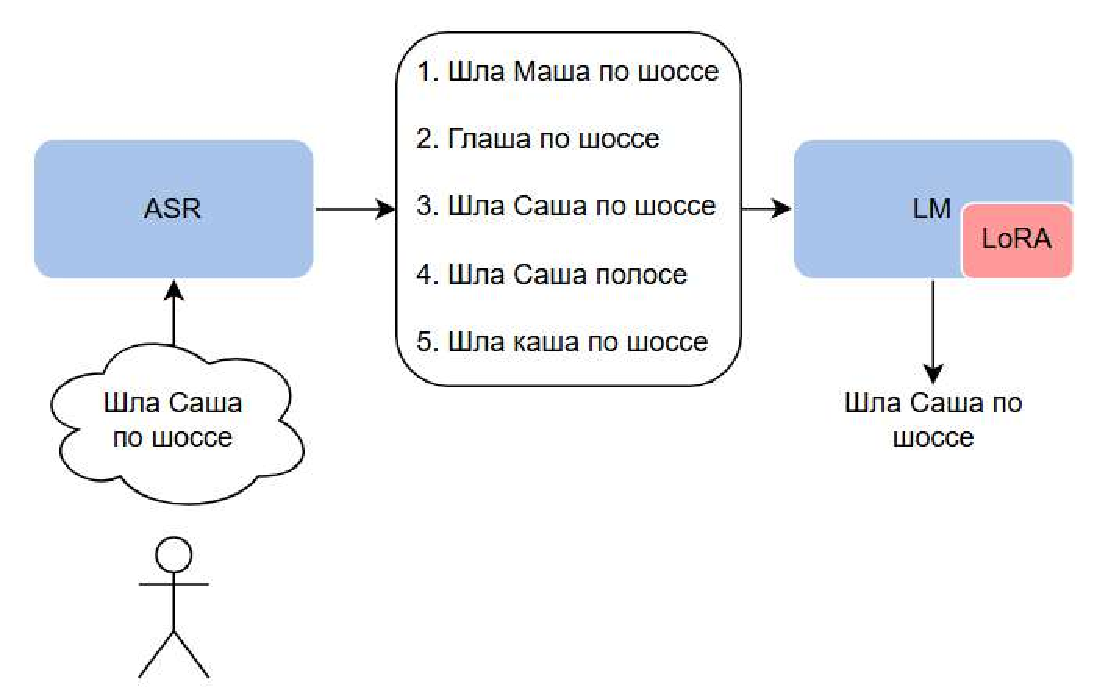
\includegraphics[width=120mm]{approach.pdf}
  \caption{Итоговая схема пайплайна.}
  \label{fig:approach}
\end{figure}

\section{Результаты}
\subsection{Основные результаты}
\begin{table}[]
\centering
\caption{Сравнение значений WER. ruT5 модель была натренирована на CV21 и RuLS}
\begin{tabular}{|c|c|ccc|}
\hline
\multirow{2}{*}{Модель}        & \multirow{2}{*}{Сеттинг}             & \multicolumn{3}{c|}{Датасет, WER}                                    \\ \cline{3-5} 
                               &                                      & \multicolumn{1}{c|}{CV21}  & \multicolumn{1}{c|}{RuLS}     & OpenSTT \\ \hline
\multirow{6}{*}{FastConformer} & Greedy                               & \multicolumn{1}{c|}{12.31} & \multicolumn{1}{c|}{38.43}    & 25.13   \\ \cline{2-5} 
                               & BeamSearch                           & \multicolumn{1}{c|}{12.26} & \multicolumn{1}{c|}{38.84}    & 25.07   \\ \cline{2-5} 
                               & LM                                   & \multicolumn{1}{c|}{9.87}  & \multicolumn{1}{c|}{37.18}    & 27.28   \\ \cline{2-5} 
                               & Greedy+Distill                       & \multicolumn{1}{c|}{13.81} & \multicolumn{1}{c|}{42.16}    & -       \\ \cline{2-5} 
                               & BeamSearch+Distill                   & \multicolumn{1}{c|}{3.82}  & \multicolumn{1}{c|}{42.10}    & -       \\ \cline{2-5} 
                               & BeamSearch+ruT5                      & \multicolumn{1}{c|}{9.75}  & \multicolumn{1}{c|}{34.32}    & 23.81   \\ \hline
\multirow{4}{*}{Whisper}       & Greedy                               & \multicolumn{1}{c|}{19.60} & \multicolumn{1}{c|}{37.89}    & 24.38   \\ \cline{2-5} 
                               & BeamSearch                           & \multicolumn{1}{c|}{18.33} & \multicolumn{1}{c|}{35.49}    & 24.19   \\ \cline{2-5} 
                               & Greedy+Distill                       & \multicolumn{1}{c|}{20.57} & \multicolumn{1}{c|}{41.40}    & -       \\ \cline{2-5} 
                               & BeamSearch+ruT5                      & \multicolumn{1}{c|}{14.32} & \multicolumn{1}{c|}{32.48}    & 23.90   \\ \hline
\end{tabular}
\label{tab:res_full}
\end{table}

Проанализируем результаты Таблицы~\ref{tab:res_full}.

\subsection{Обучение исключительно на CommonVoice}
\begin{table}[]
\centering
\caption{Сравнение значений WER. ruT5 модель была натренирована исключительно на CV21.}
\begin{tabular}{|c|c|ccc|}
\hline
\multirow{2}{*}{Модель}        & \multirow{2}{*}{Сеттинг}             & \multicolumn{3}{c|}{Датасет, WER}                                    \\ \cline{3-5} 
                               &                                      & \multicolumn{1}{c|}{CV21}  & \multicolumn{1}{c|}{RuLS}     & OpenSTT \\ \hline
\multirow{2}{*}{FastConformer} & BeamSearch                           & \multicolumn{1}{c|}{12.26} & \multicolumn{1}{c|}{38.34}    & 25.07   \\ \cline{2-5} 
                               & BeamSearch+ruT5                      & \multicolumn{1}{c|}{3.20}  & \multicolumn{1}{c|}{40.07}    & 23.38   \\ \hline
\multirow{2}{*}{Whisper}       & BeamSearch                           & \multicolumn{1}{c|}{18.33} & \multicolumn{1}{c|}{35.49}    & 24.19   \\ \cline{2-5} 
                               & BeamSearch+ruT5                      & \multicolumn{1}{c|}{4.99}  & \multicolumn{1}{c|}{38.04}    & 23.90   \\ \hline
\end{tabular}
\label{tab:res_cv_trained}
\end{table}

Взглянув на Таблицу~\ref{tab:res_cv_trained}, мы можем сделать несколько выводов.
Во-первых — подход с коррекцией текстовой расшифровки аудио показывает себя лучше всех.
Это значит, что богатые лингвистические знания модели + дообучение под нашу задачу работают отлично.
Во-вторых можно увидеть, что перенос знаний между разными ASR моделями также работает.
Так наша модель смогла в 4 раза улучшить качество распознавания для Whisper, хотя до этого она обучалась исключительно на результатах FastConformer.
Также в обоих случаях использование дистиллированной модели при сценарии жадного декодирования не принесло никакого прироста в качестве, а наоборот показало ухудшение. Причин такого падения назвать наверняка нельзя.
Можно сказать, что ASR модели, используя свои знания о языке, имеют более точное представление о правописание и пунктуации.
Или же distill модель пыталась поменять какое-то слово, которое в изменение не нуждалось, из-за чего WER вырос.

\textcolor{red}{ТАБЛИЦА С ГЕНЕРАЦИЯМИ ЧЕРИПИКНИ}

\section{Ограничения}

Мы зависим от качества распознавания ASR.
Для оценки влияния, мы намерено атаковали Whisper с помощью Projection Gradient Descent (PGD).
Это итеративный метод оптимизации, применяемый для задач с ограничениями на параметры.
Он сочетает идеи градиентного спуска с проекцией на допустимое множество.
Он является одним из самых популярных методов white-box атак на модели, то есть видов воздействия, когда у нас есть доступ к выходу модели и её архитектуре.

PGD расширяет классический градиентный спуск, добавляя шаг проекции после каждого обновления параметров.
Если градиентный спуск просто двигается в направлении антиградиента, то PGD дополнительно "проецирует" новую точку обратно на допустимое множество, если та вышла за его пределы. Это позволяет контролировать свойства модели, такие как устойчивость к атакам или физическую осмысленность параметров.
PGD решает задачу атаки итеративно, комбинируя градиентный подъём (для увеличения потерь) и проекцию (для соблюдения ограничений).
Таким образом генерируется шум на аудио.

\begin{table}[]
\centering
\caption{Эксперимент с Projected Gradient Descent white-box атакой на модель Whisper.}
\begin{tabular}{|c|c|c|}
\hline
Модель                         & Сеттинг                              & WER     \\ \hline
\multirow{2}{*}{Whisper}       & BeamSearch                           & 24.48   \\ \cline{2-3} 
                               & BeamSearch+ruT5                      & 21.34   \\ \hline
\end{tabular}
\label{tab:pgd}
\end{table}

\section{Дополнительные эксперименты}

Были проведены дополнительные эксперименты с NEFTune и текстовой аугментацией.
Поговорим сначала про NEFTune.

\subsection{NEFTune}
Он представляет собой метод регуляризации, разработанный для улучшения процесса дообучения языковых моделей.
Его ключевая особенность заключается во внесении контролируемого гауссовского шума к эмбеддингам входных токенов перед их подачей в модель на этапе обучения, что способствует повышению устойчивости и обобщающей способности модели.
Этот подход особенно эффективен при работе с ограниченными наборами данных для дообучения.

Математически это выражается как модификация исходного векторного представления через добавление случайного вектора, элементы которого распределены по нормальному закону.

\begin{equation}
  \begin{aligned}
    &\epsilon \sim Uniform(-1, 1) \\
    &X^`_{emb} = X^`_{emb} + (\frac{\alpha}{\sqrt{Ld}})\cdot\epsilon  
  \end{aligned}
  \label{eq:neftune}
\end{equation}
, где $L$ и $d$ - размерности вектора, а $\alpha$ - задаваемая величина шума.

Для успешного использования NEFTune необходимо тщательно подбирать уровень шума.
Слишком интенсивное зашумление может ухудшить качество модели, тогда как недостаточное - не даст желаемого регуляризирующего эффекта.
Оптимальные значения параметра шума обычно находятся в относительно узком диапазоне, авторы проверяли диапозон [5, 15].
Экспериментально установлено, что метод демонстрирует наибольшую эффективность при работе с небольшими наборами данных для дообучения.
Однако настройка уровня шума вместе с тем и является главным недостатком NEFTune.
Метод требует тщательного подбора параметра шума, что может увеличивать время настройки модели.
Также отмечается незначительное увеличение времени обучения из-за дополнительных операций генерации и добавления шума.

В стандартном процессе обучения по большей части ничего не меняется.
Модель продолжает использовать стандартную функцию потерь и немодифицированный алгоритм обратного распространения ошибки.
Однако перед каждым прямым проходом к входным эмбеддингам добавляется шумовой компонент, то есть эмбеддинга вычисляется его зашумленная версия.
Важно отметить, что эта операция выполняется исключительно на этапе обучения, тогда как при инференсе модель работает с исходными, незашумленными представлениями.
Такой подход обеспечивает сохранение производительности модели в рабочих условиях.

Добавление шума выполняет несколько полезных функций в процессе обучения.
Во-первых, оно действует как дополнительный регуляризатор, предотвращая переобучение модели на специфичных особенностях небольшого обучающего набора.
Во-вторых, шум способствует сглаживанию ландшафта оптимизируемой функции, помогая алгоритму избегать локальных минимумов.
В-третьих, каждый пример в эпоху обучения получает уникальную шумовую добавку, что косвенно увеличивает разнообразие обучающих данных.

По сравнению с традиционными методами регуляризации, NEFTune обладает рядом преимуществ.
В отличие от dropout, который воздействует на активации скрытых слоев, он работает непосредственно с входными представлениями.
Благодаря этому не происходит поломок графа  и перекомпиляций.
В сравнении с weight decay, который глобально ограничивает величину параметров, NEFTune обеспечивает более тонкое и адаптивное регулирование процесса обучения.
При этом метод сохраняет простоту реализации и не требует значительных вычислительных ресурсов.

\subsection{Текстовая аугментация}
Бла-бла-бла

\subsection{Результаты дополнительных экспериментов}

\begin{table}[]
\centering
\caption{Эксперимент с аугментированием гипотез с целью улучшить качество генерации.}
\begin{tabular}{|c|c|c|}
\hline
Модель                         & Сеттинг                              & WER     \\ \hline
\multirow{3}{*}{FastConformer} & BeamSearch                           & 12.26   \\ \cline{2-3} 
                               & BeamSearch+ruT5 (neft)               & 169.94  \\ \cline{2-3} 
                               & BeamSearch+ruT5 (aug)                & 71.42   \\ \hline
\multirow{3}{*}{Whisper}       & BeamSearch                           & 18.33   \\ \cline{2-3} 
                               & BeamSearch+ruT5 (neft)               & 168.90  \\ \cline{2-3} 
                               & BeamSearch+ruT5 (aug)                & 79.52   \\ \hline
\end{tabular}
\label{tab:fails}
\end{table}

\section{Анализ производительности}
По итогу можно уверенно сказать, что наш метод показал в разы лучшее качество в сравнение с другими методами и при этом затраты вычислительных ресурсов, требуемых для inference пары FastConformer + ruT5 сравнительно не велико.
В сумме обе эти модели помещаются в 3-4 Гб видеопамяти, что в современном мире является минимумом для самых низкобюджетных карт, в том числе и среди ноутбучных.

\section{Выводы}
